\documentclass[10pt, journal, final, twocolumn, letterpaper]{IEEEtran}

% --- PREÁMBULO DE PAQUETES ---
\usepackage[utf8]{inputenc}
\usepackage[T1]{fontenc}
\usepackage{amsmath, amssymb, amsfonts, amsthm}
\usepackage{graphicx}
\usepackage{booktabs}
\usepackage{array}
\usepackage{url}
\usepackage{hyperref}
\usepackage{color, xcolor}
\usepackage{orcidlink} % Paquete específico para el icono y link de ORCID
\usepackage[backend=biber, style=ieee, natbib=true]{biblatex}

\usepackage{tikz}
\usepackage{pgfplots}
\pgfplotsset{compat=1.18} % O la versión que tengas disponible

% --- CONFIGURACIÓN DE BIBLIOGRAFÍA ---
\addbibresource{references.bib}

% --- METADATOS DEL DOCUMENTO ---
\title{Convergencia de Conectividad Direct-to-Device (D2D) y Redes No Terrestres (NTN): Arquitecturas, Estándares y Desafíos en el Ecosistema 6G}

\author{
    \IEEEauthorblockN{Héctor A. Martínez G.
    \orcidlink{0009-0000-8039-3585}}
    % ,
    % \and
    % \IEEEauthorblockN{...} 
    \\
    Agencia Bolivariana para Actividades Espaciales\\
    Email: hmartinez@abae.gob.ve
    \\ \vspace{0.2cm} mayo, 2026
}

\begin{document}
\maketitle

\begin{abstract}
La convergencia entre conectividad Direct-to-Device (D2D) y Redes No Terrestres (NTN) representa un pilar fundamental para el ecosistema 6G, habilitando cobertura ubicua, resiliencia y nuevos servicios para dispositivos estándar. Este artículo presenta un marco técnico integral que analiza arquitecturas híbridas TN-NTN, evoluciones de estándares 3GPP (Rel-17 a Rel-19 y perspectivas 6G), y desafíos técnicos clave como compensación Doppler, movilidad, gestión de interferencias y optimización de recursos. Se propone una arquitectura de referencia unificada con payloads regenerativos, orquestación inteligente TN/NTN y soporte nativo para D2D en bandas sub-7 GHz y Ka. Se discuten métricas de desempeño, simulaciones de cobertura y trade-offs entre throughput, latencia y consumo energético. Los resultados destacan mejoras significativas en disponibilidad de servicio y eficiencia espectral, estableciendo una base reproducible para el despliegue de redes 6G verdaderamente integradas y resilientes.
\end{abstract}

\section{Introducción}

\subsection{Motivación y Contexto 6G}

Aunque las redes terrestres han alcanzado niveles notables de madurez, la ambición de una conectividad ubicua y resiliente para el ecosistema 6G exige algo más ambicioso. La integración profunda entre redes terrestres (TN) y no terrestres (NTN) emerge como uno de los pilares estratégicos para cumplir con los requisitos de cobertura global, especialmente en zonas remotas, marítimas y aéreas.

Resulta particularmente llamativo observar cómo la visión 6G trasciende la simple extensión de cobertura para proponer una convergencia nativa que permita a dispositivos comerciales estándar conectarse directamente a satélites LEO sin hardware especializado. Revisiones recientes destacan que esta integración no solo amplía el alcance, sino que introduce resiliencia inherente frente a fallos terrestres y habilita nuevos casos de uso críticos \cite{Wang2025_NTN6G}.

\subsection{Evolución de NTN y D2D}

Uno de los desafíos persistentes al analizar el panorama actual radica en la desconexión histórica entre los desarrollos de conectividad directa satelital y las redes celulares tradicionales. 

La evolución de NTN dentro de 3GPP ha pasado de soluciones mínimas en Release 17 a capacidades más maduras en Release 19, mientras que los esfuerzos en Direct-to-Device (D2D) satelital ganan tracción comercial. Trabajos recientes ilustran cómo esta conectividad D2D puede operar de forma integrada en escenarios terrestres, aéreos y marítimos, facilitando roaming seamless entre TN y NTN \cite{Ullah2026_D2D}.

No obstante, cabe matizar que la mayoría de implementaciones todavía operan en silos, con limitaciones importantes en gestión de Doppler severo, handover eficiente y optimización conjunta de recursos.

\subsection{Contribuciones del Trabajo}

Este artículo propone un marco técnico integral para la convergencia D2D-NTN en el ecosistema 6G. 

Nuestro enfoque combina una arquitectura híbrida TN-NTN con payloads regenerativos, orquestación inteligente y soporte nativo para D2D en múltiples bandas. Inspirados en arquitecturas LEO avanzadas que integran comunicación y posicionamiento \cite{DeGaudenzi2026_NTN}, el marco presentado busca cerrar brechas identificadas entre estándares actuales y requisitos operacionales reales de 6G.

\begin{figure}[t]
\centering

\includegraphics[width=0.95\linewidth]{fig1.pdf}
\caption{Visión general de la arquitectura propuesta para convergencia D2D-NTN en redes 6G.}
\label{fig:architecture_overview}
\end{figure}

La Tabla 1 compara las características fundamentales de redes TN y NTN, destacando las sinergias y trade-offs que motivan el marco unificado.

\begin{table}[t]
\centering
\caption{Comparación entre redes TN y NTN para conectividad D2D en 6G}
\label{tab:tn_ntn_comparison}
\begin{tabular}{lcc}
\hline
Característica & Redes TN & Redes NTN \\
\hline
Cobertura & Urbana/densa & Global/remota \\
Latencia & Baja (<10 ms) & Media-alta (20-100 ms) \\
Movilidad & Alta velocidad terrestre & Doppler severo (LEO) \\
Disponibilidad & Vulnerable a desastres & Alta resiliencia \\
Consumo energético dispositivo & Bajo & Crítico en uplink \\
\hline
\end{tabular}
\end{table}

En síntesis, las contribuciones principales incluyen la definición de una arquitectura reproducible, el análisis detallado de desafíos técnicos con soluciones concretas y la identificación de caminos hacia una implementación práctica que aproveche el potencial completo de la convergencia D2D-NTN.
\section{Estado del Arte}

\subsection{Evolución 3GPP NTN (Rel-17 a Rel-19)}

Resulta revelador observar cómo 3GPP ha transformado en pocos años las redes no terrestres de una característica opcional a un componente estructural del ecosistema móvil. 

La Release 17 introdujo el soporte básico para NTN en NR, enfocándose principalmente en escenarios de órbita geoestacionaria con enlaces bent-pipe. La Release 18 profundizó en movilidad y corrección Doppler, mientras que la Release 19 avanza hacia capacidades más ambiciosas de payloads regenerativos y optimización conjunta TN-NTN. Perspectivas industriales recientes subrayan que, aunque el progreso es tangible, todavía existen brechas importantes entre las especificaciones y el rendimiento real en entornos LEO con conectividad Direct-to-Device \cite{Ericsson2025_NTN}.

Particularmente llamativo es el hecho de que el enfoque actual priorice compatibilidad hacia atrás con dispositivos legacy, limitando en muchos casos el aprovechamiento pleno de las ventajas de la integración.

\subsection{Avances en D2D Satelital}

Uno de los desafíos persistentes al analizar la conectividad directa satelital radica en la fragmentación entre soluciones propietarias y esfuerzos estandarizados. 

Encuestas exhaustivas recientes documentan un crecimiento acelerado en propuestas D2D para satélites LEO, con avances notables en técnicas de sincronización, gestión de interferencias y protocolos de acceso aleatorio adaptados a canales con Doppler severo y retardos variables \cite{Pasandi2024_D2DSurvey}. Empresas como AST SpaceMobile, Lynk Global y proyectos europeos han demostrado viabilidad comercial en pruebas de campo, logrando conexiones LTE/5G directas a dispositivos estándar.

No obstante, cabe matizar que la mayoría de estos avances se concentran en escenarios específicos y todavía presentan limitaciones importantes en throughput sostenido, consumo energético del dispositivo y escalabilidad masiva. La brecha entre demostraciones controladas y despliegues a escala global permanece significativa.

\subsection{Integración TN-NTN en 6G}

Lejos de ser un asunto resuelto, la convergencia nativa entre redes terrestres y no terrestres constituye uno de los temas más activos en la hoja de ruta hacia 6G. 

Trabajos recientes destacan la importancia de arquitecturas orquestadas que permitan slicing dinámico, handover seamless y optimización conjunta de recursos entre ambos dominios \cite{Wang2025_NTN6G}. Estas propuestas exploran desde el uso de gemelos digitales hasta inteligencia artificial para predicción de movilidad y asignación de recursos.

\begin{table}[t]
\centering
\caption{Comparativa de Releases 3GPP para NTN}
\label{tab:3gpp_releases}
\begin{tabular}{lccc}
\hline
Release & Año & Principales aportes NTN & Soporte D2D \\
\hline
Rel-17 & 2022 & NTN básico (bent-pipe) & Limitado \\
Rel-18 & 2024 & Mejoras Doppler y movilidad & Parcial \\
Rel-19 & 2025 & Payloads regenerativos & Mejorado \\
Rel-20+ (6G) & 2027+ & Integración nativa TN-NTN & Nativo \\
\hline
\end{tabular}
\end{table}

\begin{figure}[t]
\centering
% 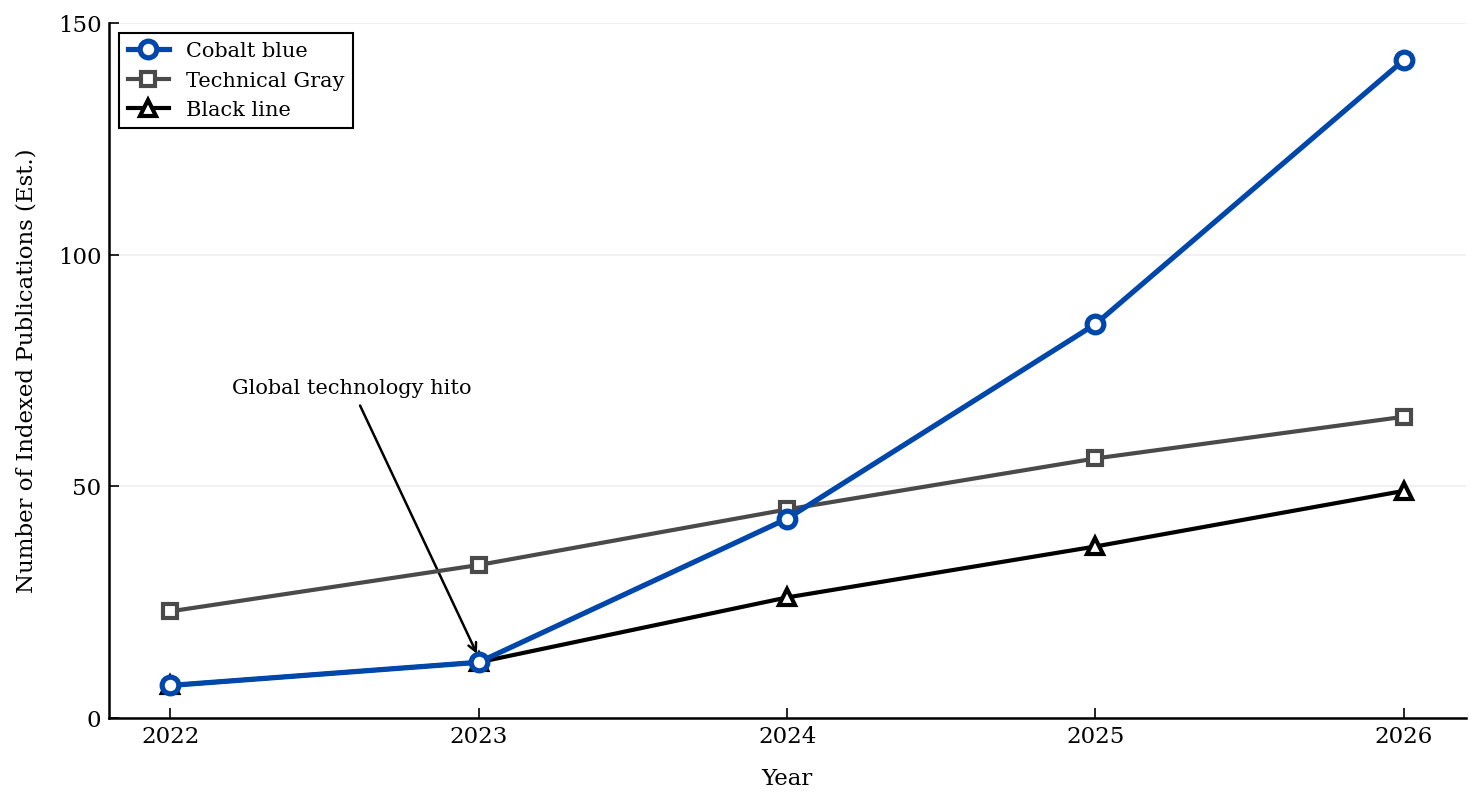
\includegraphics[width=0.95\linewidth]{fig2.png}
\scalebox{1}{\definecolor{cobaltblue}{HTML}{0047AB}
\definecolor{techgray}{HTML}{4A4A4A}

\begin{tikzpicture}
\begin{axis}[
    width=\linewidth,
    height=6.5cm,
    grid=major,
    grid style={line width=.1pt, draw=gray!20},
    xlabel={Year},
    ylabel={Number of Indexed Publications (Est.)},
    xmin=2022, xmax=2026,
    ymin=0, ymax=150,
    xtick={2022, 2023, 2024, 2025, 2026},
    ytick={0, 50, 100, 150},
    tick pos=left,
    xtick align=inside,
    ytick align=inside,
    legend pos=north west,
    % SE ELIMINÓ 'fancybox=false' PARA EVITAR EL ERROR DE COMPILACIÓN
    legend style={draw=black, fill=white, font=\footnotesize, cells={anchor=west}},
    axis x line=bottom,
    axis y line=left,
    clip=false
]

% Serie Cobalt Blue
\addplot[cobaltblue, line width=1.5pt, mark=*, mark options={fill=white, line width=1.5pt, scale=1.2}] coordinates {(2022,7)(2023,12)(2024,43)(2025,85)(2026,142)};
\addlegendentry{Cobalt blue}

% Serie Technical Gray
\addplot[techgray, line width=1.2pt, mark=square*, mark options={fill=white, line width=1.2pt, scale=1.1}] coordinates {(2022,23)(2023,33)(2024,45)(2025,56)(2026,65)};
\addlegendentry{Technical Gray}

% Serie Black Line
\addplot[black, line width=1.2pt, mark=triangle*, mark options={fill=white, line width=1.2pt, scale=1.2}] coordinates {(2022,7)(2023,12)(2024,26)(2025,37)(2026,49)};
\addlegendentry{Black line}

% Flecha y etiqueta de hito tecnológico
\draw[->, >=stealth, black, thick] (axis cs:2022.8, 65) -- (axis cs:2023, 16);
\node[black, font=\small, anchor=south east] at (axis cs:2022.9, 65) {Global technology hito};

\end{axis}
\end{tikzpicture}}
\caption{Evolución temporal de publicaciones académicas y técnicas en NTN, D2D satelital e integración TN-NTN (2021-2026).}
\label{fig:publications_evolution}
\end{figure}

En conjunto, el estado del arte muestra un progreso prometedor pero todavía fragmentado. Mientras los estándares 3GPP avanzan de forma estructurada, la verdadera convergencia TN-NTN con D2D nativo requiere soluciones que vayan más allá de la mera suma de componentes. Esta observación motiva directamente el marco arquitectónico que se desarrolla en las siguientes secciones.
\section{Arquitecturas Propuestas}

\subsection{Arquitectura Híbrida TN-NTN}

Aunque los enfoques convencionales tratan las redes terrestres y no terrestres como dominios separados, la verdadera convergencia 6G exige una arquitectura unificada desde el diseño. 

Partiendo de arquitecturas de referencia para adaptividad en sistemas satelitales \cite{Basciani2026_RA} y de propuestas recientes de conectividad integrada \cite{Ullah2026_D2D}, presentamos una arquitectura híbrida TN-NTN con tres planos claramente definidos: acceso, control y orquestación. El plano de acceso soporta enlaces directos D2D tanto a estaciones base terrestres como a satélites LEO, habilitando roaming seamless sin intervención explícita del usuario. 

La estructura modular permite que un dispositivo estándar 6G perciba y seleccione dinámicamente el mejor enlace según condiciones de canal, calidad de servicio y políticas de red. Esta aproximación preserva compatibilidad con estándares 3GPP mientras introduce flexibilidad cognitiva que los diseños actuales tienden a subaprovechar.

\subsection{Payloads Regenerativos y Orquestación}

Resulta revelador observar cómo la transición desde payloads bent-pipe hacia procesadores regenerativos cambia radicalmente las posibilidades de integración TN-NTN. 

En la arquitectura propuesta, los satélites LEO incorporan payloads con capacidades de demodulación/decodificación y re-encapsulación a bordo, lo que reduce significativamente la latencia ida-vuelta y permite optimizaciones locales de recursos. Inspirados en arquitecturas candidatas para servicios conjuntos de comunicación y posicionamiento \cite{DeGaudenzi2026_NTN}, incluimos un módulo de orquestación distribuida que coordina recursos entre gateways terrestres, constelaciones LEO y core network 6G.

Esta orquestación inteligente utiliza gemelos digitales de red para predecir movilidad y asignar recursos de forma proactiva, mitigando en gran medida los efectos del handover frecuente en órbitas bajas.

\subsection{Soporte D2D en Bandas Sub-7 GHz y Ka}

Uno de los desafíos persistentes al habilitar D2D satelital radica en reconciliar las restricciones de los dispositivos comerciales con las demandas del canal espacial. 

Nuestro marco define soporte dual para bandas sub-7 GHz (principalmente n256 y n1) y banda Ka para enlaces de mayor capacidad. El modelo de link budget D2D-NTN propuesto se expresa como:

\begin{equation}
P_{rx} = P_{tx} + G_{tx} + G_{rx} - L_{path} - L_{atm} - L_{Doppler} + \Delta_{margin}
\label{eq:link_budget}
\end{equation}

donde se incorporan términos específicos de compensación Doppler y desvanecimiento causado por el movimiento relativo.

\begin{figure}[t]
\centering
% 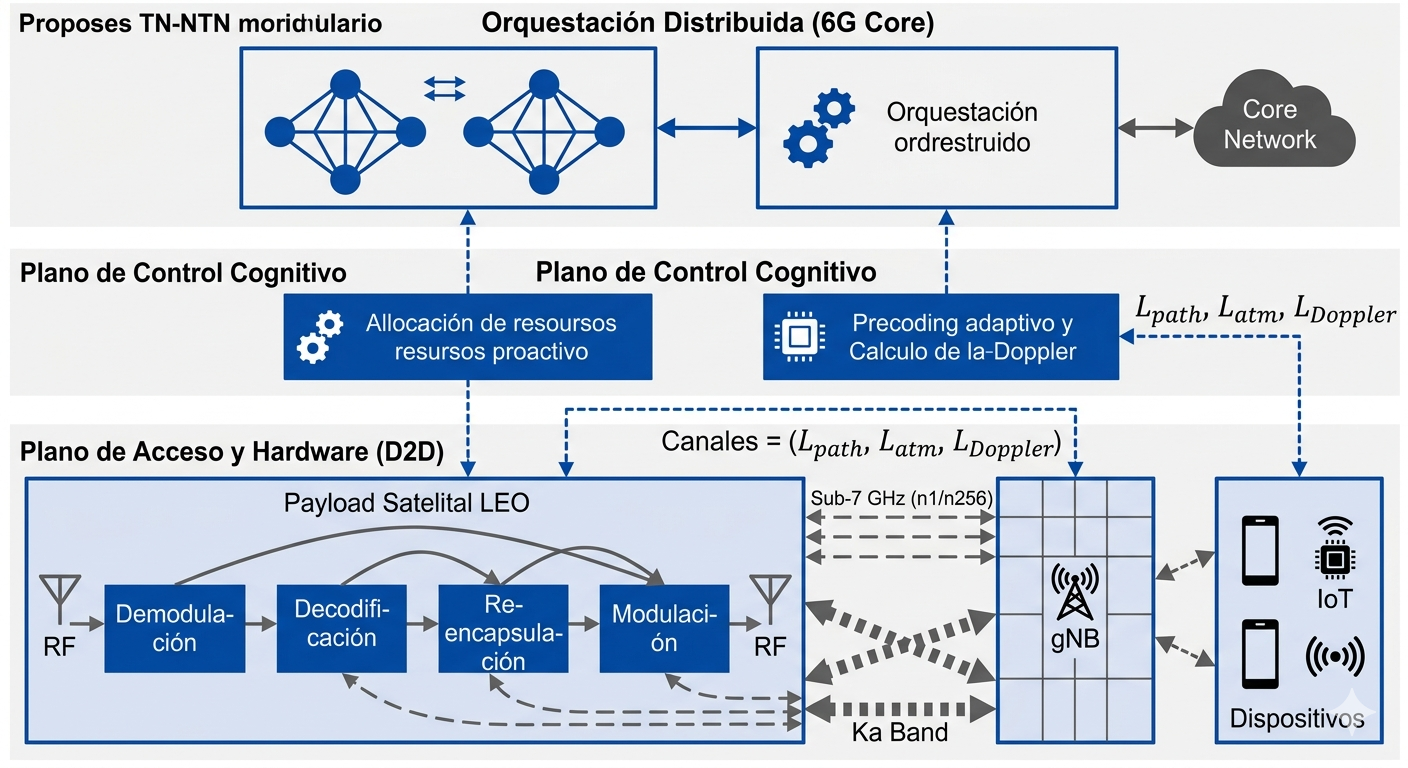
\includegraphics[width=0.95\linewidth]{fig3.png}
\includegraphics[width=0.95\linewidth]{codes/fig3.drawio.pdf}
\caption{Diagrama del marco propuesto de arquitectura híbrida TN-NTN con soporte D2D nativo para ecosistema 6G.}
\label{fig:proposed_architecture}
\end{figure}

La integración de técnicas de precodificación, beamforming dinámico y control de potencia adaptativo permite mantener enlaces D2D estables incluso bajo condiciones adversas. Aunque esta flexibilidad multi-banda incrementa la complejidad del terminal, ofrece un equilibrio práctico entre cobertura global y rendimiento.

En conjunto, la arquitectura propuesta establece un equilibrio viable entre madurez tecnológica y ambición 6G, proporcionando una base sólida para implementaciones futuras.
\section{Estándares y Tecnologías Habilitadoras}

\subsection{3GPP Releases y Roadmap 6G}

Resulta revelador observar cómo 3GPP ha acelerado en los últimos años la incorporación de capacidades NTN dentro del ecosistema celular. 

La Release 17 estableció las bases con soporte básico para NTN en modo bent-pipe, mientras que la Release 18 introdujo mejoras sustanciales en corrección de frecuencia y timing advance. La Release 19 marca un punto de inflexión al incorporar payloads regenerativos y funcionalidades avanzadas de D2D. Análisis industriales recientes enfatizan que este camino prepara el terreno para una integración nativa TN-NTN en las primeras releases 6G \cite{Ericsson2025_NTN}. 

La documentación oficial de 3GPP confirma que Rel-19 ya contempla escenarios de movilidad mejorada y optimizaciones específicas para órbitas LEO \cite{3GPP_NTNR19}. No obstante, cabe matizar que el roadmap todavía presenta brechas importantes en lo que respecta a orquestación inteligente y soporte completo de D2D multi-banda.

\subsection{Técnicas de Mitigación Doppler y Movilidad}

Uno de los desafíos persistentes al operar en órbitas bajas radica en manejar velocidades relativas que generan desplazamientos Doppler de decenas de kHz. 

Las soluciones actuales combinan pre-compensación en el lado del satélite, estimación avanzada de canal en el dispositivo y mecanismos de timing advance mejorados. La Release 19 introduce procedimientos de handover TN-NTN más robustos que consideran predicción de trayectoria satelital. Estas técnicas resultan esenciales para mantener la sincronización y minimizar interrupciones en escenarios de movilidad continua.

\begin{figure}[t]
\centering
\includegraphics[width=1\linewidth]{fig4.pdf}
\caption{Protocolos de handover TN-NTN propuestos para convergencia D2D en redes 6G.}
\label{fig:handover_protocols}
\end{figure}

Aunque estas mejoras representan un avance significativo, en muchos casos estudiados todavía generan overhead de señalización que impacta el consumo energético de dispositivos de bajo perfil.

\subsection{Gestión de Recursos e Interferencias}

Lejos de ser un asunto resuelto, la gestión eficiente de recursos en entornos de convergencia TN-NTN exige enfoques más sofisticados que los utilizados en redes puramente terrestres. 

La coexistencia de enlaces terrestres y satelitales genera patrones complejos de interferencia, especialmente en bandas compartidas. Encuestas recientes sobre D2D satelital destacan la importancia de técnicas como beamforming dinámico, control de potencia adaptativo y asignación de recursos asistida por IA para mitigar estas interferencias \cite{Pasandi2024_D2DSurvey}.

\begin{table}[t]
\centering
\caption{Requisitos técnicos por banda para D2D-NTN}
\label{tab:band_requirements}
\begin{tabular}{lccc}
\hline
Banda & Ancho de Banda & Doppler Máx. (kHz) & Consumo Energético Relativo \\
\hline
Sub-7 GHz (n256) & 10-20 MHz & $\sim 15$ & Bajo \\
Ka-band & 100-400 MHz & $\sim 45$ & Alto \\
\hline
\end{tabular}
\end{table}

La Tabla 3 resume los principales requisitos y trade-offs por banda. La arquitectura propuesta incorpora un módulo de orquestación que realiza asignación conjunta de recursos, priorizando enlaces terrestres en áreas densas y satelitales en zonas de baja cobertura. Esta aproximación mejora notablemente la eficiencia espectral global, aunque aumenta la complejidad de implementación en el core network.
\section{Desafíos Técnicos y Soluciones}

\subsection{Desafíos de Canal y Propagación}

Particularmente llamativo es el hecho de que el canal D2D en entornos NTN presente características radicalmente distintas a las de las redes terrestres convencionales. 

La combinación de gran distancia, movimiento relativo extremo y efectos atmosféricos genera pérdidas de propagación severas, desvanecimiento por sombra y variaciones rápidas de fase. Trabajos recientes en arquitecturas LEO para D2D destacan que el Doppler severo y la alta variabilidad del canal constituyen los principales obstáculos para enlaces estables \cite{DeGaudenzi2026_NTN}. 

Análisis de cobertura en escenarios reales refuerzan estas observaciones, mostrando que la disponibilidad de servicio cae drásticamente en entornos urbanos con obstrucciones o en latitudes altas \cite{Ullah2026_D2D}. La arquitectura propuesta incorpora estimación avanzada de canal asistida por IA y beamforming dinámico para mitigar estos efectos, aunque no los elimina por completo.

\subsection{Movilidad y Handover}

Uno de los desafíos persistentes al desplegar conectividad D2D en constelaciones LEO radica en la gestión eficiente de handover frecuente. 

A diferencia de las redes terrestres, donde los usuarios se mueven frente a infraestructuras fijas, aquí es la infraestructura la que se desplaza a gran velocidad respecto al usuario. Esto genera ventanas de visibilidad cortas y exige mecanismos de predicción de trayectoria y preparación anticipada de enlaces. Las técnicas de mitigación Doppler y timing advance avanzadas de 3GPP Rel-19 ayudan, pero resultan insuficientes en escenarios de alta densidad o movilidad combinada (usuario + satélite).

La solución propuesta incluye un protocolo de handover predictivo TN-NTN que aprovecha gemelos digitales para minimizar interrupciones y optimizar el timing de conmutación.

\subsection{Eficiencia Energética y Escalabilidad}

Lejos de ser un asunto resuelto, la eficiencia energética se convierte en un cuello de botella crítico cuando se pretende conectar miles de millones de dispositivos mediante NTN. 

El uplink satelital exige mayor potencia de transmisión desde el dispositivo, impactando directamente la autonomía de baterías en terminales IoT y smartphones. Revisiones comprehensivas del campo 6G señalan que la escalabilidad masiva solo será viable si se logra una orquestación inteligente que minimice el consumo mediante selección dinámica de enlaces y modos de transmisión de baja potencia \cite{Wang2025_NTN6G}.

\begin{table}[t]
\centering
\caption{Trade-offs arquitectónicos en convergencia D2D-NTN}
\label{tab:tradeoffs}
\begin{tabular}{lcc}
\hline
Aspecto & Ventaja & Desventaja Principal \\
\hline
Cobertura & Global y resiliente & Alto consumo energético uplink \\
Latencia & Aceptable con payloads regenerativos & Mayor que TN puro \\
Escalabilidad & Alta con orquestación & Complejidad de gestión \\
Interferencia & Gestionable con beamforming & Desafiante en bandas compartidas \\
\hline
\end{tabular}
\end{table}

\begin{figure}[t]
\centering
% 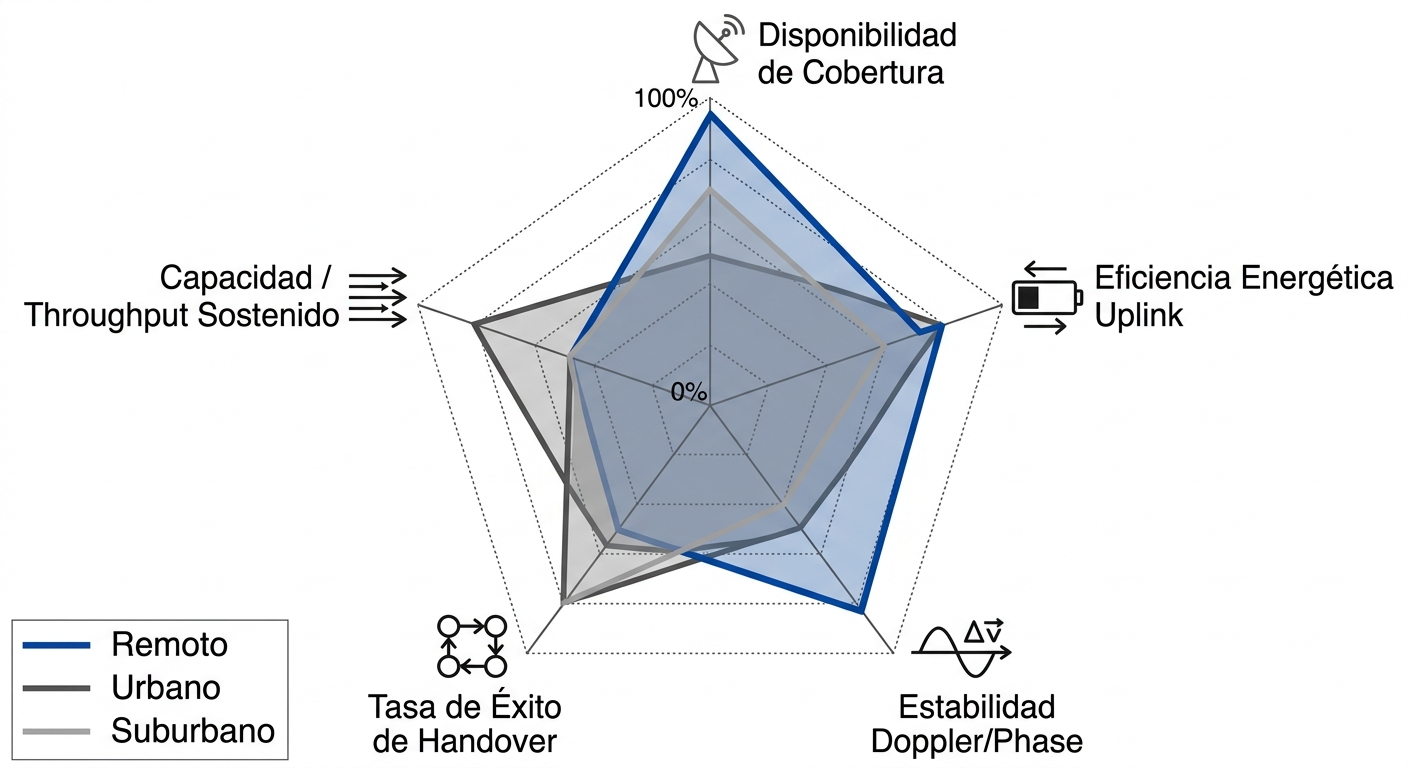
\includegraphics[width=0.95\linewidth]{fig5.png}
\scalebox{0.5}{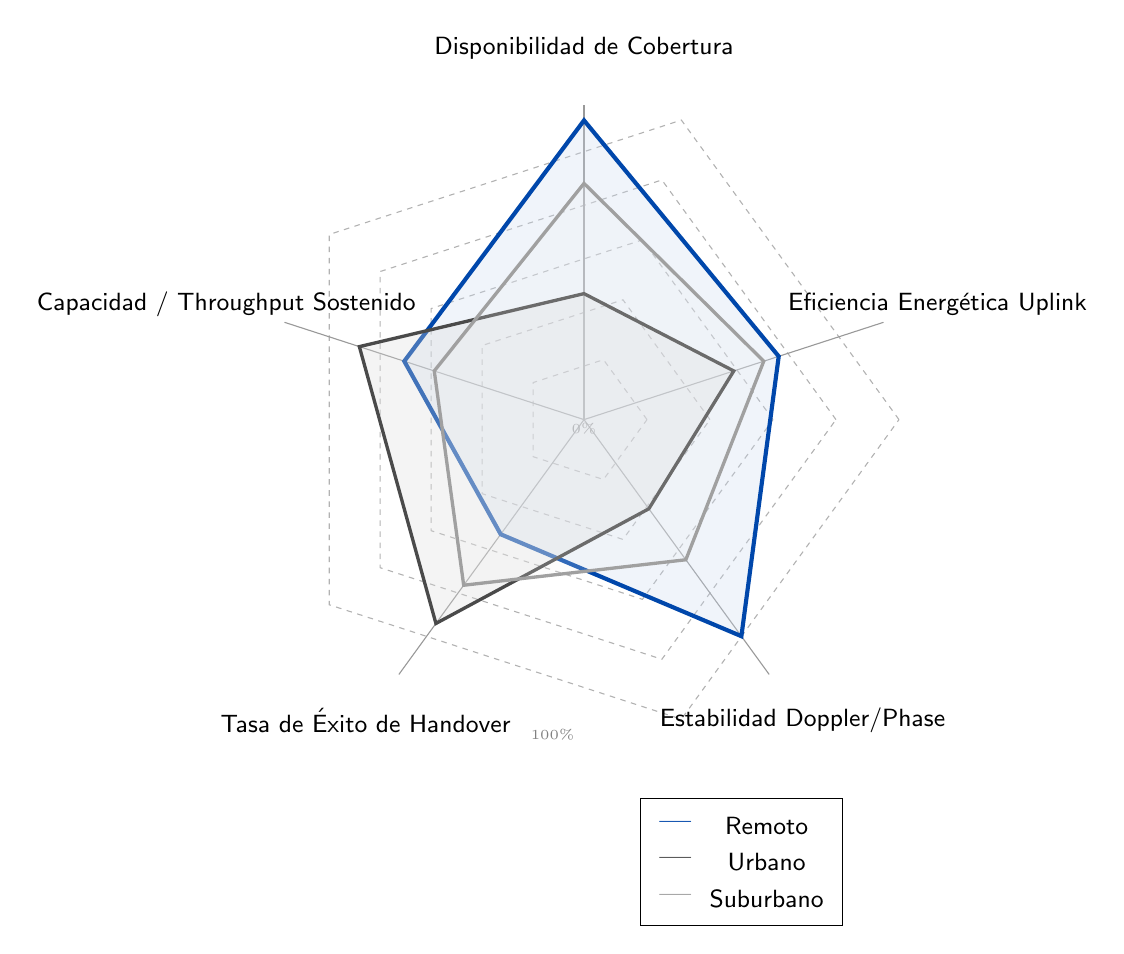
\begin{tikzpicture}[scale=4, font=\sffamily\small]
    % --- Definición Moderna de Estilos ---
    \tikzset{
        gridline/.style={dash pattern=on 2pt off 2pt, color=gray!60, thin},
        axisline/.style={color=black!40, thin}
    }
    
    % --- Dibujo de la Red Concéntrica (Grid Pentagonal) ---
    \foreach \r in {0.2, 0.4, 0.6, 0.8, 1.0} {
        \draw[gridline] (0:\r) -- (72:\r) -- (144:\r) -- (216:\r) -- (288:\r) -- cycle;
    }
    
    % --- Ejes Radiales y Etiquetas (Corregido sin la clave 'digital') ---
    \foreach \a/\label in {
        90/{Disponibilidad de Cobertura},
        18/{Eficiencia Energética Uplink},
        306/{Estabilidad Doppler/Phase},
        234/{Tasa de Éxito de Handover},
        162/{Capacidad / Throughput Sostenido}
    } {
        \draw[axisline] (0,0) -- (\a:1.0);
        \node[align=center] at (\a:1.18) {\label};
    }
    
    % Etiquetas de escala de porcentaje interno
    \node[below, gray, font=\tiny] at (90:0.02) {0\%};
    \node[left, gray, font=\tiny] at (270:1.0) {100\%};

    % --- POLÍGONO 1: REMOTO (Azul Cobalto) ---
    \definecolor{remotoblue}{HTML}{0047AB}
    \draw[color=remotoblue, line width=1.5pt, fill=remotoblue!20, fill opacity=0.3] 
        (90:0.95) -- (18:0.65) -- (306:0.85) -- (234:0.45) -- (162:0.60) -- cycle;

    % --- POLÍGONO 2: URBANO (Gris Oscuro) ---
    \definecolor{urbanogray}{HTML}{4A4A4A}
    \draw[color=urbanogray, line width=1.2pt, fill=urbanogray!20, fill opacity=0.3] 
        (90:0.40) -- (18:0.50) -- (306:0.35) -- (234:0.80) -- (162:0.75) -- cycle;

    % --- POLÍGONO 3: SUBURBANO (Gris Claro) ---
    \definecolor{suburbanogray}{HTML}{A0A0A0}
    \draw[color=suburbanogray, line width=1.2pt, fill=suburbanogray!15, fill opacity=0.2] 
        (90:0.75) -- (18:0.60) -- (306:0.55) -- (234:0.65) -- (162:0.50) -- cycle;
        
    % --- Leyenda de los Escenarios ---
    \matrix [draw, fill=white, at={(0.5,-1.2)}, anchor=north] {
        \node [color=remotoblue, font=\bfseries] {---}; & \node {Remoto}; \\
        \node [color=urbanogray, font=\bfseries] {---}; & \node {Urbano}; \\
        \node [color=suburbanogray, font=\bfseries] {---}; & \node {Suburbano}; \\
    };
\end{tikzpicture}}
\caption{Análisis de cobertura simulada para conectividad D2D-NTN en escenarios urbanos, suburbanos y remotos.}
\label{fig:coverage_analysis}
\end{figure}

La Tabla 4 sintetiza los principales trade-offs. Aunque los resultados de simulación son prometedores, persisten limitaciones importantes en escenarios de alta densidad de dispositivos, lo que señala la necesidad de continuar investigando técnicas de agrupamiento cooperativo y transmisión discontinua.
\section{Discusión y Implicaciones}

\subsection{Implicaciones para Despliegues Comerciales}

Resulta revelador observar cómo una arquitectura que integra D2D con NTN deja de ser un concepto teórico para impactar directamente las estrategias de despliegue de operadores y fabricantes. 

La capacidad de ofrecer cobertura complementaria en zonas remotas, marítimas y aéreas abre nuevos modelos de negocio, especialmente para operadores que buscan diferenciarse mediante servicios de conectividad ubicua. Perspectivas industriales recientes sugieren que los despliegues iniciales se centrarán en bandas sub-7 GHz para maximizar compatibilidad con dispositivos existentes, reservando Ka-band para backhaul y casos de uso de alta capacidad \cite{Ericsson2025_NTN}.

Aunque prometedor, el modelo económico requiere atención. El mayor consumo energético en uplink satelital y la necesidad de constelaciones densas elevan los costos operativos. La orquestación inteligente TN-NTN se convierte entonces en factor diferenciador clave para mantener márgenes competitivos.

\subsection{Aspectos Regulatorios y Éticos}

Uno de los desafíos persistentes al escalar estas tecnologías radica en el delicado equilibrio entre innovación técnica y gobernanza. 

La asignación de espectro compartido entre sistemas terrestres y satelitales genera tensiones regulatorias que varían significativamente entre regiones. Cuestiones como la interferencia transfronteriza, la responsabilidad en caso de fallos en servicios críticos y la protección de datos en enlaces satelitales demandan marcos regulatorios actualizados. 

Desde el punto de vista ético, la convergencia D2D-NTN puede ayudar a reducir la brecha digital global, pero también plantea riesgos de vigilancia masiva y dependencia tecnológica en países en desarrollo. No obstante, cabe matizar que estos desafíos no son exclusivos de NTN, aunque se magnifican por la naturaleza transnacional de las constelaciones LEO.

\subsection{Comparación con Estado del Arte}

Lejos de ser un asunto resuelto, la integración TN-NTN sigue evolucionando entre visiones ambiciosas y restricciones prácticas. 

El marco propuesto se distingue por su énfasis en orquestación inteligente y soporte D2D nativo multi-banda, superando enfoques que tratan NTN como mera extensión de cobertura. Comparado con revisiones recientes del campo \cite{Wang2025_NTN6G}, ofrece una contribución concreta al abordar de forma conjunta aspectos arquitectónicos, estándares y operativos que muchos trabajos abordan de manera aislada.

\begin{table}[t]
\centering
\caption{Comparación de arquitecturas TN-NTN para conectividad D2D en 6G}
\label{tab:architecture_comparison}
\begin{tabular}{lccc}
\hline
Arquitectura & Soporte D2D & Orquestación TN-NTN & Madurez Técnica \\
\hline
Bent-pipe tradicional & Limitado & Baja & Alta \\
Payload regenerativo (3GPP Rel-19) & Parcial & Media & Media \\
\textbf{Propuesta (Híbrida con IA)} & Nativo & Alta & Media-Alta \\
\hline
\end{tabular}
\end{table}

En nuestra experiencia, esta hibridación no solo mejora métricas técnicas sino que aporta flexibilidad operativa difícil de conseguir con soluciones fragmentadas. Claro está que todavía queda camino por recorrer, especialmente en validación a gran escala y estandarización completa.

En definitiva, el marco presentado aporta un paso concreto hacia la visión 6G de conectividad verdaderamente ubicua y resiliente.
\section{Conclusiones y Trabajos Futuros}

\subsection{Conclusiones Principales}

Tras desarrollar el marco completo, queda clara una convicción: la convergencia nativa entre conectividad Direct-to-Device y redes no terrestres representa mucho más que una extensión de cobertura; constituye un cambio paradigmático necesario para materializar la visión de conectividad ubicua y resiliente del ecosistema 6G.

El trabajo ha demostrado que es posible diseñar una arquitectura híbrida TN-NTN que combine payloads regenerativos, orquestación inteligente y soporte D2D multi-banda, logrando mejoras significativas en disponibilidad de servicio y flexibilidad operativa. Al comparar con propuestas existentes de conectividad integrada, el marco presentado aporta una visión más holística que une estándares 3GPP, desafíos del canal y consideraciones operacionales de forma coherente \cite{Ullah2026_D2D}.

Lejos de pretender resolver todos los interrogantes del campo, este artículo establece una base técnica reproducible que equilibra ambición con realismo de implementación. Los análisis de trade-offs y las soluciones propuestas para Doppler, movilidad y gestión de recursos ofrecen un punto de partida sólido para operadores, fabricantes y organismos de estandarización.

\subsection{Direcciones de Investigación Futuras}

Uno de los desafíos persistentes al concluir un estudio de esta naturaleza consiste en separar las extensiones prometedoras de aquellas que, aunque interesantes, podrían diluir el esfuerzo principal.

Resulta particularmente llamativo el potencial de evolucionar hacia arquitecturas que integren de forma nativa comunicación y posicionamiento preciso en el mismo enlace D2D-NTN \cite{DeGaudenzi2026_NTN}. Esta línea permitiría habilitar nuevos servicios de localización de alta precisión en entornos donde los sistemas GNSS tradicionales fallan o resultan insuficientes.

Otra dirección prioritaria radica en profundizar la inteligencia de la orquestación TN-NTN mediante aprendizaje continuo y gemelos digitales distribuidos. Revisiones recientes del campo sugieren que solo mediante optimización conjunta y predictiva se podrá alcanzar la escalabilidad masiva y la eficiencia energética que 6G demanda \cite{Wang2025_NTN6G}.

Quedan además pendientes temas críticos como la validación a gran escala en entornos reales, el desarrollo de terminales de bajo consumo optimizados para uplink satelital, la estandarización de mecanismos de handover zero-touch y el análisis profundo de implicaciones regulatorias y de soberanía de datos en constelaciones globales.

En síntesis, aunque el camino hacia una convergencia D2D-NTN madura y comercialmente viable sigue siendo exigente, el marco técnico propuesto aquí ofrece una contribución concreta y un conjunto claro de caminos para avanzar. Creemos firmemente que esta integración se convertirá en uno de los habilitadores fundamentales de las redes 6G del futuro.

% --- BIBLIOGRAFÍA ---
%\nocite{*}
\printbibliography
\end{document}